\chapter{Exploring Language Model}
\label{chapter:langModel}
%%===========================================================================%%
\section{Analysis of Vocubalry stats}
\fixme{Upto 1 page: mostly fresh writing}
Visualizations of vocabulary and learned word-vectors

\section{Additional Feature Inputs to Language Model}

In the basic model, both visual features and the word embeddings are fed through
the same input matrices, $W_{ix}$.
%%
The visual features are thus present in the network inputs only in the zeroth
round of iteration.
%%
This was proposed in~\cite{Vinyals_2015_CVPR} as a solution to prevent
overfitting. 
%%
But in our experiments with the COCO data set, we have found out that this is
not necessary and better models can be trained by letting the LSTM have access
to the visual features throughout the caption generation process.

This requires adding to the LSTM cell a new input path which we refer to as the
\emph{persist} features.
%%
This input plays the same role as $x(t)$ in
equations~(\ref{eqn:lstmstrt})--(\ref{eqn:lstmend}), but it has its own set of
embedding weights.
%%
This allows the model to treat the word embeddings and the image features
differently and thus makes the model more powerful.
%%
Note that we can input different visual features in the \emph{init} and
\emph{persist} paths thereby allowing the model to learn simultaneously from two
different sources.

%%===========================================================================%%
\section{Deeper model, residual connections }
\fixme{Upto 1 page: From ACMMM paper}
%% ---------------------------------------------------------------------------
We also train language models with multiple LSTM layers.
%%
Only the first LSTM layer receives the feature inputs and the higher LSTM layers
take their input $x(t)$ from the previous layer in the network.
%%
The recurrent connections from a network's outputs back to its inputs exist only
within an LSTM layer and not across the layers.
%%
Softmax is applied at the output of the last LSTM layer only.
%%

Our last modification is adding multiple LSTM layers with residual connections
after each layer as proposed in~\cite{He2015} for convolutional neural networks.
%%
These residual connections, shown in Figure~\ref{fig:lstmlang}, seem to improve
the training convergence speed greatly.
%%
We have also found out that the use of residual connections produces
significantly lower values for both the training cost function and the model
perplexity, as will be detailed in Section~\ref{sec:experiments}.

%%===========================================================================%%
\section{Class based Factorization}
\fixme{Upto 1 pages: fresh writing }
%%===========================================================================%%
\section{Bi-Directional LSTMs ????}
\fixme{Not sure yet: fresh writing }
%%===========================================================================%%
\section{Ensembling Techniques}
%%----------------------------------%%
Using the many different image features and LSTM architectures available we can
train a set of different language models. 
%%
When examining the pool of captions generated by such models for a set of
images, we have found out that different models tend to generate the best
captions for different images.
%%
If one could evaluate the suitability of a given caption for a given image, one
could possibly pick out the best candidate from the pool and achieve better
results than with any single model.

Thus our idea here is to train a new network model whose task is to pick out the
best candidate from the candidate set, given an input image. 
%%
The model takes as input the gCNN image feature and an input sentence and
computes a similarity metric between the sentence and the image. 
%%
The ensemble model is trained discriminatively, in contrast to the the language
models which have been trained generatively.

For this purpose we use a convolutional network to encode the sentences and the
cosine similarity measure to evaluate the similarity between the encoded
sentence and the image feature vector. 
%%
The approach is detailed in the following sections.

%% --------------------------------------
\subsection{MERT}
\fixme{1 or 2 paragraphs: fresh writing }
%%----------------------------------%%
\subsection{CMME}
\fixme{1 or 2 paragraphs: fresh writing }

Another method is to pick the best candidate among the pool of captions
generated by the ensemble independently.
%%
For this, we can look at the log-probability assigned to the sentence by the
generating model.
%%
But it is not fair to compare these log-probabilities as different models might
have different biases.
%%

Instead, we can get each model to rate the sentences generated by the other
models.
%%
This can be done by running the network in training mode with the candidate
sentence playing the role of the reference caption.
%%
This will give us the log-probability assigned by the model to the candidate
sentence.
%%

Thus we get N (no. of models) log probability scores for each candidate
sentence.
%%
We can take the best candidate as the one with the highest average score.
%%
We refer to this technique as Combining Multiple models with Mutual Evaluation
(CMME).
%%
This technique is similar to peer-review model and is most effective if each
model in the ensemble is fairly good, but with specializations in slightly
different parts of the dataset.
%%

%%----------------------------------%%
\subsection{CNN Evaluator}
\fixme{1 page: from report}

The convolutional network we use to encode sentences is based on the
paper~\cite{kim:2014:CNNsent}, where it is used for sentence sentiment
prediction.
%%
Figure~\ref{fig:CNNEval} shows the block diagram of our CNN-based
evaluator.  
%%
Here, the input sentence is represented as a sequence of word vectors,
which are either statically initialized with some standard word vector
encodings, such as GloVe~\cite{pennington2014glove} or
word2vec~\cite{mikolov2013distributed}, or learned during the training
phase.
%%
These word vectors are fed into a convolutional neural network which
computes an encoding of the sentence.

To compute the similarity between the image and the sentence encoding,
the image feature vector is first projected into same representation
space using a projection matrix.
%%
The similarity is then computed between the projected image vector and
the sentence encoding to give a match score between the input image
and the candidate sentence.

\begin{figure*}[t] 
  \centering
  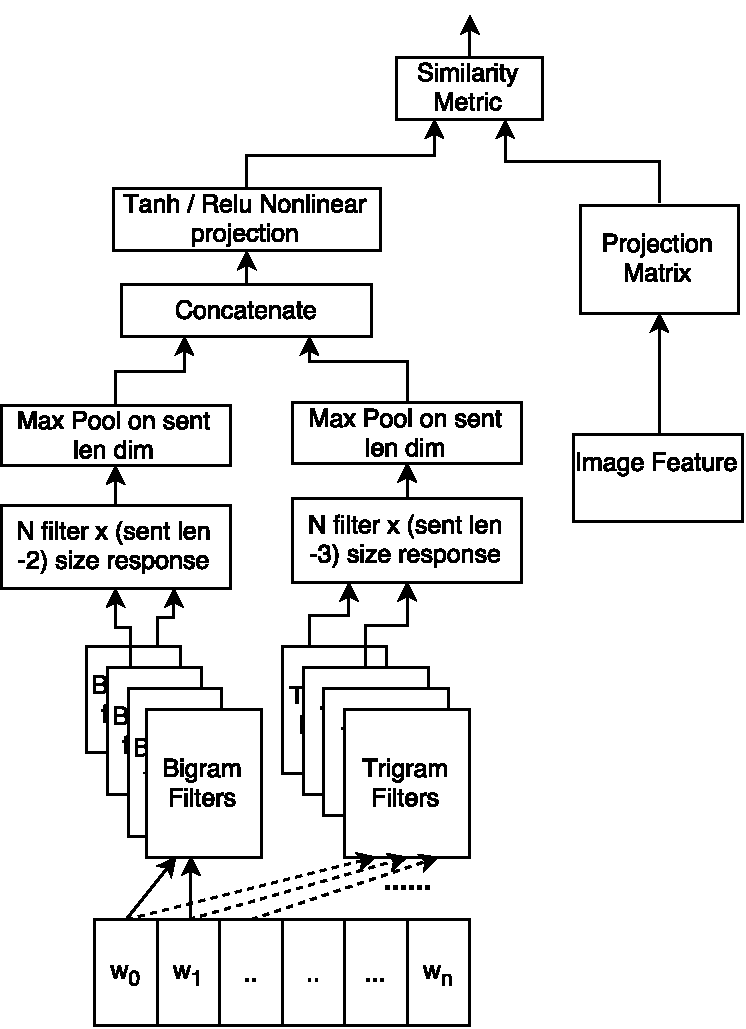
\includegraphics[width=0.5\textwidth]{./images/CnnEval.pdf} 
  \caption{CNN based evaluator network to compute the similarity between 
    an image and a caption.}
  \label{fig:CNNEval} 
\end{figure*}

% Convolutional network on sentences

The first layer in the CNN consists of convolutional filters of
different sizes.  
%%
All the filters operate over entire word vectors, but vary in the
number of words they cover, i.e., each filter is of the size
$N_{\text{gram}} \times N_{\text{word vec dim}}$. 
%%
We can thus have filters operating over bigrams, trigrams, etc.
%%
Specifically, our model has filters with bigrams, trigrams, 4-grams and
5-grams. 
%%
Additionally, we use many filters of any given size and so the total
number of filters in the models can be written as
$N_{\text{filt}} \cdot N_{\text{filt type}}$.

The filter outputs are max-pooled, which reduces the filter response
over entire sentence into a single scalar, i.e., its maximum
response. 
%%
We can therefore think of each filter as looking for a specific
n-gram, disregarding its location within the sentence.
%%
These pooled outputs are concatenated and then projected to the
desired vector size to produce the final sentence encoding.

%% --------------------------------------

\subsubsection{Training the Evaluator Network}

The evaluator network is trained to assign a high score for the
correct or the best caption and a lower scores for other captions.
%%
This is done by letting the network, for each training set image $I$,
to score its ground truth caption, $S^+$, and $k$ negative samples,
$S_i^-, i=1,\ldots,k$, drawn randomly from the ground truth captions
of other images.
%%
Now the training cost function $C$ is devised to maximize the score for
the positive sample and to minimize it for the negative samples. 
%%
This is achieved by applying a softmax on the scores of this batch
(one positive and $k$ negative samples) and maximize the softmax score
of the positive sample:
%%
\begin{align}
  \label{eq:cnnprob} 
  P(S^+|S^-,I) &= \frac{\exp(-f(S^+,I))}{\exp(-f(S^+,I)) +
           \sum\limits_i^k{\exp(-f(S_i^- ,I))}} \\
  C &= -\log P(S^+|S^-,I) \;.
\end{align}
%%
Equation~(\ref{eq:cnnprob}) shows this computation with $f(S,I)$
representing the similarity metric between the sentence candidate $S$
and image $I$.
%%
In our current method, we use the cosine similarity between the two
vectors for the purpose of $f(S,I)$.

%% --------------------------------------

\subsubsection{Utilizing the Evaluator Network}

Once trained, we can then use the evaluator network to compute the
similarity between each candidate in the pool of captions and the
image feature vector. 
%%
The candidate with the highest similarity is chosen as the output
caption from the ensemble for the image.

%% ===========================================================================
%%----------------------------------%%
\subsection{BiLstm Evaluator}
\fixme{0.5 page: fresh writing}
